\documentclass[border=10pt]{standalone}
\usepackage[svgnames]{xcolor}
\usepackage{amsmath}
\usepackage{pgfplots}
\pgfplotsset{compat=newest}
\usepackage[sfdefault]{FiraSans}
\usepackage{FiraMono}
\renewcommand*\familydefault{\sfdefault}
\begin{document}
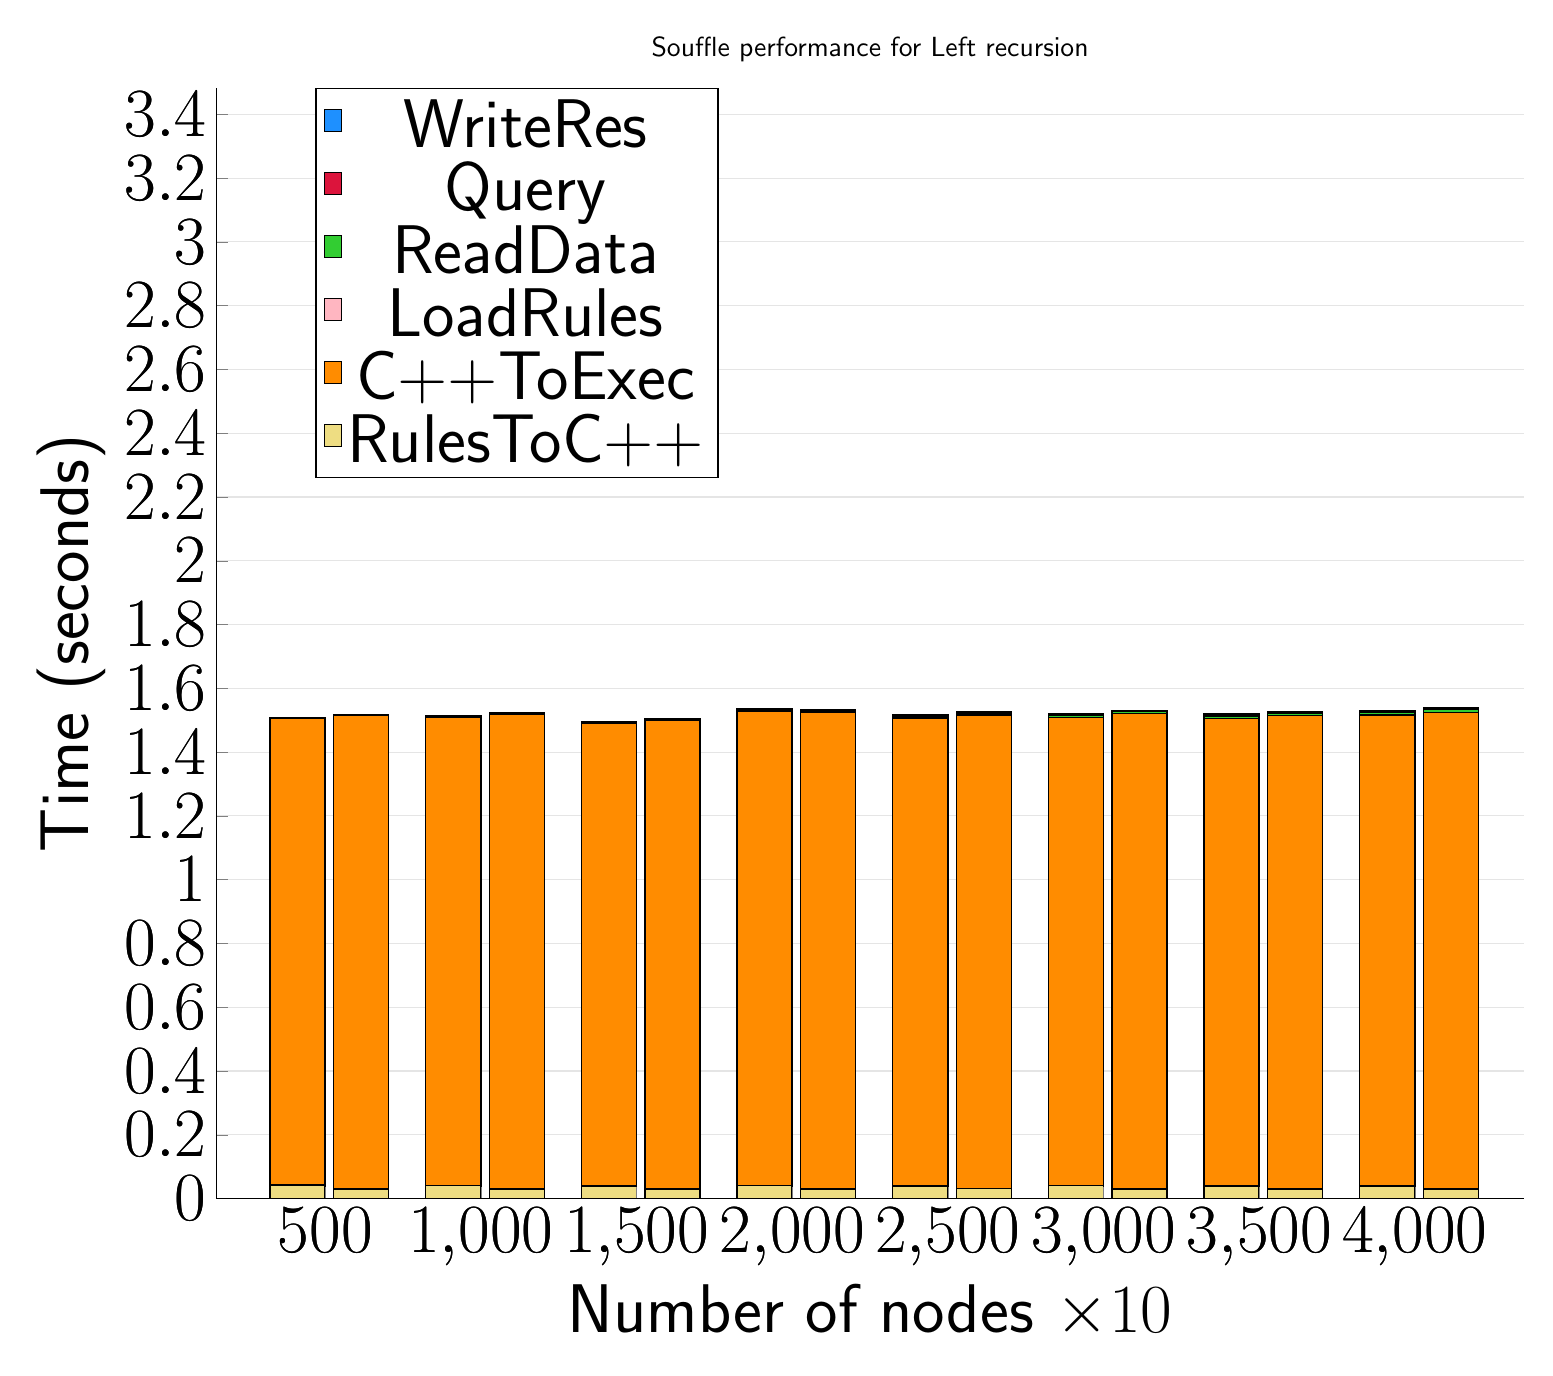
\begin{tikzpicture}
\begin{axis}[
   ybar stacked,
   title={Souffle performance for Left recursion},
   bar shift=-10pt,
   width=1.5\textwidth,
   bar width=0.7cm,
   ymajorgrids, tick align=inside,
   major grid style={draw=gray!20},
   xtick=data,
   ymin=0, ymax=3.4829999923706056,
   axis x line*=bottom,
   axis y line*=left,
   enlarge x limits=0.1,
   legend style={
       at={(0.23, 1)},
       anchor=north,
       legend columns=1,
       font=\Huge,
   },
   ylabel={Time (seconds)},
   xlabel={Number of nodes $\times 10$},
   label style={font=\Huge},
   tick label style={font=\Huge},
]
\addlegendimage{fill=DodgerBlue, draw=black, line width=0.2pt}
\addlegendentry{WriteRes}
\addlegendimage{fill=Crimson, draw=black, line width=0.2pt}
\addlegendentry{Query}
\addlegendimage{fill=LimeGreen, draw=black, line width=0.2pt}
\addlegendentry{ReadData}
\addlegendimage{fill=LightPink, draw=black, line width=0.2pt}
\addlegendentry{LoadRules}
\addlegendimage{fill=DarkOrange, draw=black, line width=0.2pt}
\addlegendentry{C++ToExec}
\addlegendimage{fill=LightGoldenrod, draw=black, line width=0.2pt}
\addlegendentry{RulesToC++}
\addplot +[fill=LightGoldenrod, draw=black, line width=0.5pt] coordinates {
    (500, 0.04200000762939453)
    (1000, 0.040999984741210936)
    (1500, 0.03899998664855957)
    (2000, 0.04100003242492676)
    (2500, 0.039999961853027344)
    (3000, 0.04100000858306885)
    (3500, 0.039999961853027344)
    (4000, 0.04000003337860107)
};
\addplot +[fill=DarkOrange, draw=black, line width=0.5pt] coordinates {
    (500, 1.4640000343322754)
    (1000, 1.4680000066757202)
    (1500, 1.4509999990463256)
    (2000, 1.4869999647140504)
    (2500, 1.4670000314712524)
    (3000, 1.4680000066757202)
    (3500, 1.4660000324249267)
    (4000, 1.4759999752044677)
};
\addplot +[fill=LightPink, draw=black, line width=0.5pt] coordinates {
    (500, 7.454590000000001e-05)
    (1000, 0.00010171689999999998)
    (1500, 0.0001111751)
    (2000, 0.00011107090000000001)
    (2500, 8.377920000000001e-05)
    (3000, 6.89958e-05)
    (3500, 0.0001216583)
    (4000, 0.00011071669999999998)
};
\addplot +[fill=LimeGreen, draw=black, line width=0.5pt] coordinates {
    (500, 0.0011316596000000001)
    (1000, 0.0024249329999999998)
    (1500, 0.0034061870000000006)
    (2000, 0.004433474)
    (2500, 0.0053014429999999986)
    (3000, 0.0060620660000000005)
    (3500, 0.007721982999999999)
    (4000, 0.008458058000000001)
};
\addplot +[fill=Crimson, draw=black, line width=0.5pt] coordinates {
    (500, 0.00043816250000000003)
    (1000, 0.0010553331)
    (1500, 0.001543301)
    (2000, 0.001953026)
    (2500, 0.0024637039999999997)
    (3000, 0.0028420509999999995)
    (3500, 0.003627188)
    (4000, 0.0043409469999999995)
};
\addplot +[fill=DodgerBlue, draw=black, line width=0.5pt] coordinates {
    (500, 0.0003957081)
    (1000, 0.0008095830999999999)
    (1500, 0.0008605203)
    (2000, 0.0010806002999999998)
    (2500, 0.0012002473)
    (3000, 0.001311229)
    (3500, 0.001609872)
    (4000, 0.0017201500000000002)
};
\end{axis}
\begin{axis}[
   ybar stacked,
   bar shift=13pt,
   width=1.5\textwidth,
   bar width=0.7cm,
   ymajorgrids, tick align=inside,
   major grid style={draw=none},
   xtick=data,
   ymin=0, ymax=3.4829999923706056,
   axis x line*=none,
   axis y line*=none,
   enlarge x limits=0.1,
   label style={font=\Huge},
   tick label style={font=\Huge},
]
\addplot +[fill=LightGoldenrod, draw=black, line width=0.5pt] coordinates {
    (500, 0.030000000000000006)
    (1000, 0.030000000000000006)
    (1500, 0.030000000000000006)
    (2000, 0.030000000000000006)
    (2500, 0.031000000000000007)
    (3000, 0.030000000000000006)
    (3500, 0.030000000000000006)
    (4000, 0.030000000000000006)
};
\addplot +[fill=DarkOrange, draw=black, line width=0.5pt] coordinates {
    (500, 1.486)
    (1000, 1.4890000000000003)
    (1500, 1.4699999999999998)
    (2000, 1.496)
    (2500, 1.4860000000000002)
    (3000, 1.491)
    (3500, 1.485)
    (4000, 1.4949999999999999)
};
\addplot +[fill=LightPink, draw=black, line width=0.5pt] coordinates {
    (500, 7.41e-05)
    (1000, 0.000101)
    (1500, 0.00011060000000000002)
    (2000, 0.0001104)
    (2500, 8.319999999999999e-05)
    (3000, 6.860000000000001e-05)
    (3500, 0.0001209)
    (4000, 0.00011)
};
\addplot +[fill=LimeGreen, draw=black, line width=0.5pt] coordinates {
    (500, 0.001131)
    (1000, 0.0024238)
    (1500, 0.0034053)
    (2000, 0.0044318)
    (2500, 0.0052959)
    (3000, 0.0060579)
    (3500, 0.0077147)
    (4000, 0.008284999999999999)
};
\addplot +[fill=Crimson, draw=black, line width=0.5pt] coordinates {
    (500, 0.0004376999999999999)
    (1000, 0.0010538)
    (1500, 0.0015428)
    (2000, 0.0019511)
    (2500, 0.0024622000000000003)
    (3000, 0.0028393000000000003)
    (3500, 0.003624)
    (4000, 0.0041826)
};
\addplot +[fill=DodgerBlue, draw=black, line width=0.5pt] coordinates {
    (500, 0.00037520000000000007)
    (1000, 0.0006571000000000001)
    (1500, 0.0008213)
    (2000, 0.0010425)
    (2500, 0.0011975000000000002)
    (3000, 0.001309)
    (3500, 0.0016054000000000003)
    (4000, 0.0016965)
};
\end{axis}
\end{tikzpicture}

\end{document}
